\documentclass{article}
\usepackage[english, italian]{babel}
\selectlanguage{italian}
\usepackage[utf8x]{inputenc}
\usepackage[T1]{fontenc}
\usepackage{graphicx}
\usepackage[colorinlistoftodos]{todonotes}
\usepackage[colorlinks=true, allcolors=tudelftblue]{hyperref} %sets hyperlink colour
\usepackage{caption}
\usepackage{subcaption}
\usepackage{xcolor}
\usepackage{roboto} % for Roboto Slab font
\usepackage{float}
\usepackage{titling} 
\usepackage{blindtext}\usepackage{titlesec}
\usepackage[square,sort,comma,numbers]{natbib}
\usepackage[colorinlistoftodos]{todonotes}
\usepackage{tikz}
\usepackage{geometry}
\usepackage{sectsty}
\usepackage{amsmath}
\usepackage{tikzpagenodes}
\usepackage{booktabs}
\usepackage{listings}
\lstdefinelanguage{json}{
    basicstyle=\ttfamily\small,
    numbers=left,
    numberstyle=\tiny\color{gray},
    stepnumber=1,
    numbersep=8pt,
    showstringspaces=false,
    breaklines=true,
    frame=lines,
    backgroundcolor=\color{gray!10},
    literate=
     *{0}{{{\color{blue}0}}}{1}
      {1}{{{\color{blue}1}}}{1}
      {2}{{{\color{blue}2}}}{1}
      {3}{{{\color{blue}3}}}{1}
      {4}{{{\color{blue}4}}}{1}
      {5}{{{\color{blue}5}}}{1}
      {6}{{{\color{blue}6}}}{1}
      {7}{{{\color{blue}7}}}{1}
      {8}{{{\color{blue}8}}}{1}
      {9}{{{\color{blue}9}}}{1}
      {:}{{{\color{red}:}}}{1}
      {,}{{{\color{red},}}}{1}
      {\{}{{{\color{black}\{}}}{1}
      {\}}{{{\color{black}\}}}}{1}
      {[}{{{\color{black}[}}}{1}
      {]}{{{\color{black}]}}}{1},
}
\lstdefinelanguage{MongoDBShell}{
    basicstyle=\ttfamily\small,
    numbers=left,
    numberstyle=\tiny\color{gray},
    stepnumber=1,
    numbersep=8pt,
    showstringspaces=false,
    breaklines=true,
    frame=lines,
    backgroundcolor=\color{gray!10},
    keywordstyle=\color{blue}\bfseries,
    stringstyle=\color{red},
    commentstyle=\color{green!70!black},
    morekeywords={use, db, show, insert, find, update, delete, createCollection, drop, aggregate},
}
\lstdefinelanguage{Python}{
    basicstyle=\ttfamily\small,
    numbers=left,
    numberstyle=\tiny\color{gray},
    stepnumber=1,
    numbersep=8pt,
    showstringspaces=false,
    breaklines=true,
    frame=lines,
    backgroundcolor=\color{gray!10},
    keywordstyle=\color{blue}\bfseries,
    stringstyle=\color{red},
    commentstyle=\color{green!70!black},
    morekeywords={import, from, class, def, return, if, elif, else, for, while, in, try, except, with, as, pass, break, continue, True, False, None},
}

\geometry{a4paper, margin=2cm}
\definecolor{unimorered}{RGB}{209,65,36}
\definecolor{unimoregrey}{RGB}{99,102,106}
\definecolor{tudelftblue}{RGB}{0, 80, 162}
\allsectionsfont{\color{black}} %sets colour for all headers
\usepackage{helvet}
\renewcommand{\familydefault}{\sfdefault}
\sectionfont{\fontfamily{RobotoSlab-TLF}\selectfont}
%%%%%%%%%%%%%%%%%%%%%%%%%%%%%%%%%%%%%%%%%%%%%%%%%%%%%%%%%
\begin{document}

\input{titlepage}

%%% Create a table of contents
\tableofcontents
\newpage

\addcontentsline{toc}{section}{Abstract}
\section*{Abstract}

In questo report si esporrà il funzionamento e le caratterisch di MongoDB, un database NoSQL. In particolare verranno presentate le funzonalità di questo database,
il modo in cui si possono memorizzare i dati e come effettuare le principali operazioni CRUD (Create, Read, Update, Delete). 
In questo specifico caso di utilizzo MongoDB è stato utilizzato per memorizzare i dati di un 
negozio musicale, riadattando la struttura nativa relazionale del database in una struttura NoSQL più
adatta a MongoDB. Tutte le operazioni sono state effettuate tramite python, utilizzando la libreria pymongo.
Infine è stata sviluppata una interfaccia grafica in streamlit per interrogare in modo dinamico il database,
sia per la parte musicale che per la parte amministrativa e di vendite. Il codice sorgente è disponibile
al repository GitHub disponibile al link fornito.



\section{MongoDB}

\subsection{Introduzione}

MongoDB è un database NoSQL, ossia un database non relazionale che archivia i dati in modo flessibile. MongoDB offre un servizio su Cloud, MongoDB Atlas
e una versione MongoDB Community, installabile sulla propria macchina in locale. Per gli scopi di questo progetto è stato installato
MongoDB Community in locale. MongoDB è pensato per essere scalato orizzontalmente, distribuendo i dati su più macchine e con varie repliche, per garantire
alta disponibilità e tolleranza ai guasti. 

Un record in MongoDB è un documento, ossia una struttura dati composta da coppie di chiavi a valori; questi valori potrebbero 
essere a loro volta documenti, oppure vettori o valori. La struttura di un documento è simile a quella di un oggetto JSON,
ossia un oggetto JavaScript che rappresenta una struttura dati composta da coppie di chiavi a valori. In particolare MongoDB salva i documenti in formato BSON, ossia una rappresentazione binaria dei file JSON. 
Un esempio di documento è il seguente:

\begin{lstlisting}[language=json, caption={Esempio di JSON}]
    {
        "Nome": "Paolo",
        "Professione": Studente",
        "TitoliDiStudio": ["Diploma", "Laurea Triennale"],
        "Indirizzo": {
            "Via": "Campi"
            "NumeroCivivo": "213/b",
            "Cap": 41125,
            "Citta": "Modena"
        },
        "Anni": 24,
    }
\end{lstlisting}


L'utilizzo di documenti come record per il salvataggio di dati ha diversi vantaggi, infatti documenti di questo tipo corrispondono 
al tipo nativo di dati in molti linguaggi di programmazione. Inoltre la possibilità di annidare documenti e di inserire array 
come valori permette di avere strutture di dati che diminuiscono le operazioni di join.
MongoDB memorizza i documenti in \textit{collezioni}, ossia l'equivalente delle tabelle in database relazionali. Inoltre MongoDB
supporta anche:
\begin{itemize}
    \item \textbf{Viste di sola lettura}: viste virtuali basate su una query che mostrano una finestra sui dati di una collezione esistente, aggiornata automaticamente ogni volta che viene consultata la finestra
    \item \textbf{Viste materializzate su richiesta}: una tabella o una collezione che memorizza i risultati di una query per migliorare le prestazioni, non vengono aggiornate automaticamente ma solo manualmente o tramite script
\end{itemize}

\subsection{Modalità di utilizzo}
MongoDB può ssere utilizzato in diversi modi, tra cui:
\begin{itemize}
    \item MongoDB Shell
    \item MongoDB Compass
    \item MongoDB Atlas
    \item Driver MongoDB
\end{itemize}

\textbf{MongoDB Shell} è un'interfaccia a riga di comando che permette di interagire con il database, eseguire query
e comandi di amministrazione. La shell risulta utile per eseguire operazioni rapide e testare comandi, ma non è adatta
all'uso in produzione.

\textbf{MongoDB Compass} è un'interfaccia grafica che permette di esplorare i dati, eseguire query e visualizzare i risultati,
fornisce uno strumento utile per analizzare i dati e per eseguire operazioni di amminitrazione, ma non è adatta per l'uso in produzione.

\textbf{MongoDB Atlas} è un servizio di database as a service (DBaaS) che permette di creare e gestire cluster MongoDB
in cloud. Atlas offre funzionalità avanzate come il backup automatico, la scalabilità automatica e la sicurezza integrata previo pagamento,
ma mette a disposizione anche un piano gratuito con una capacità massima di 512 MB e alcune limitazioni per backup e replica.

\textbf{Driver MongoDB} sono librerie che permettono di interagire con MongoDB da diversi linguaggi di programmazione,
 come Python, Java, Node.js e altri. I driver offrono un'interfaccia per eseguire operazioni CRUD e per gestire
  le connessioni al database. Per questo progetto è stato utilizzato il driver \textbf{pymongo} per Python. 
  Utilizzare un driver significa potersi appoggiare a un linguaggio di programmazione per costruire query ed effettuare operazioni
  in modo dinamico e automatico.

\subsection{Operazioni CRUD}

Le operazioni CRUD (Create, Read, Update, Delete) sono le operazioni fondamentali per interagire con un database. In
    MongoDB queste operazioni vengono eseguite tramite metodi specifici. Di seguito sono riportati alcuni esempi di operazioni CRUD
    utilizzando MongoDB Shell. Supponiamo di avere in locale MongoDB Compass e MongoDB Shell installati, allora le istruzioni a seguire
    permettono di creare un database \textit{Scuola} e due collezioni, \textit{Studenti} e \textit{Professori}.

    \begin{lstlisting}[language=MongoDBShell, caption={Esempio di operazioni CRUD in MongoDB Shell}]
    use Scuola
    db.createCollection(
        "Studenti", {
        validator: {
            $jsonSchema: {
                bsonType: "object",
                title: "Validazione dell'oggetto Studente",
                required: ["Id", "Nome", "Cognome"],
                properties: {
                    Id: { bsonType: "int" },
                    Nome: { bsonType: "string" },
                    Cognome: { bsonType: "string" },
                    DataDiNascita: { bsonType: "date"}
                }
            }
        }
    } )
    db.Studenti.createIndex({ "Id": 1 }, { unique: true })
    db.createCollection(
        "Professori", {
        validator: {
            $jsonSchema: {
                bsonType: "object",
                title: "Validazione dell'oggetto Studente",
                required: ["Id", "Nome", "Cognome"],
                properties: {
                    Id: { bsonType: "int" },
                    Nome: { bsonType: "string" },
                    Cognome: { bsonType: "string" },
                    DataDiNascita: { bsonType: "date"}
                }   
            }   
        }
    } )
    db.Professori.createIndex({ "Id": 1 }, { unique: true })
    \end{lstlisting}

Le operazioni CRUD mostrate creano un database Scuola, due collezioni, Studenti e Professori, e 
definiscono uno schema per la validazione dei documenti: è richiesto che siano inseriti almeno un Id, 
un Nome e un Cognome. Inoltre viene richiesto, tramite la creazione un indice, che gli Id siano univoci
nelle rispettive collezioni. Se durante una fase di insert non vengono soddisfatti questi
requisiti, MongoDB non permette di inserire il documento e restituisce un errore.

\subsubsection{Insert}
MongoDB permette di inserire documenti tramite dei metodi, \textit{insert\_one} e \textit{insert\_many}, che nello specifico inseriscono uno
o più documenti in una collezione. Di seguito sono riportati alcuni esempi di inserimento di documenti.

\begin{lstlisting}[language=MongoDBShell, caption={Esempio di insert in MongoDB}]
    db.Studenti.insertOne({
        Id: 2,
        Nome: "Luca",
        Cognome: "Rossi",
        DataDiNascita: ISODate("2000-05-15T00:00:00Z")
    })
    db.Studenti.insertMany([
        {
            Id: 2,
            Nome: "Stefano",
            Cognome: "Verdi",
            DataDiNascita: ISODate("2000-05-15T00:00:00Z")
        },
        {
            Id: 3,
            Nome: "Anna",
            Cognome: "Bianchi",
            DataDiNascita: ISODate("1999-11-20T00:00:00Z")
        },
        {
            Id: 4,
            Nome: "Marco",
            Cognome: "Galli",
            DataDiNascita: ISODate("2001-01-10T00:00:00Z")
        }
    ])

\end{lstlisting}
In modo analogo si possono inserire dei documenti nella collezione Professori.

\subsubsection{Delete}
MongoDB permette di eliminare documenti tramite i metodi \textit{delete\_one} e \textit{delete\_many}, che eliminano uno
o più documenti in una collezione. Di seguito sono riportati alcuni esempi di eliminazione di documenti.

\begin{lstlisting}[language=MongoDBShell, caption={Esempio di delete in MongoDB}]
    db.Studenti.deleteOne({ Id: 2 })
    db.Studenti.deleteMany({ Nome: "Marco" })
    db.Studenti.deleteMany({ Nome: { $in: ["Marco", "Luca"] } })
    db.Studenti.deleteMany({ Nome: { $nin: ["Marco", "Luca"] } })

\end{lstlisting}
Il primo comando elimina il documento con Id 2, il secondo elimina tutti i documenti in cui il campo "Nome" è "Marco", il terzo elimina
tutti i documenti in cui il campo "Nome" è "Marco" o "Luca", mentre il quarto elimina tutti i documenti in cui il campo "Nome" non è "Marco" o "Luca".

\subsubsection{Update}

MongoDB permette di aggiornare documenti tramite i metodi \textit{update\_one} e \textit{update\_many}, che aggiornano uno
o più documenti in una collezione. Durnte gli update vengono spessi usate pipeline di aggregazione, che permettono di concatenare
più azioni una dopo l'altra. In seguito verranno approfondite le pipeline di aggregazione, per il momento sono riportati alcuni
esempi di aggiornamento di documenti.

\begin{lstlisting}[language=MongoDBShell, caption={Esempio di update in MongoDB}]
    db.Studenti.updateOne(
        { Id: 2 },
        { $set: { Nome: "Marco" } }
    )
    db.Studenti.updateMany(
        { Nome: "Marco" },
        { $set: { Nome: "Luca" } }
    )
    db.Studenti.updateMany(
        { Corso: { $exists: false } },
        { $set: { Corso: "Matematica" } }   
    )
\end{lstlisting}
Il primo comando aggiorna il documento con Id 2, cambiando il campo Nome in Marco, il secondo cambia il campo Nome in Luca per tutti i documenti
in cui il campo Nome è Marco, mentre il terzo aggiorna tutti i documenti in cui il campo Corso non esiste, aggiungendo il campo Corso con valore Matematica.

\subsubsection{Read}
MongoDB permette di leggere documenti tramite i metodi \textit{findOne}, \textit{find} che restituiscono uno o più documenti in una collezione.
Entrambi i metodi prendono in input un filtro che permette di specificare quali documenti si vogliono leggere, espressi in formato JSON, e un 
parametro di proiezione che permette di specificare quali campi di vogliono restituire e con quale nome, sempre in formato JSON. Di seguito sono riportati alcuni
esempi di lettura di documenti.
\begin{lstlisting}[language=MongoDBShell, caption={Esempio di read in MongoDB}]
    db.Studenti.find()
    db.Studenti.find({ Id: 2 })
    db.Studenti.find({ Corso: "Matematica" })
    db.Studenti.find(
        { Corso: "Matematica" },
        { Nome: 1, Cognome: 1, _id: 0 }
    )
\end{lstlisting}
Il primo comando restituisce tutti i documenti nella collezione Studenti, il secondo restituisce il documento con Id 2, il terzo restituisce tutti i documenti in cui il campo Corso è Matematica, mentre il quarto restituisce solo i campi Nome e Cognome dei documenti in cui il campo Corso è Matematica, escludendo il campo \_id.

\subsection{Aggregazione}

MongoDB mette a disposizione un potente framwork di aggregazione che permette di eseguire operazioni complesse sui dati, come filtri,
ordinamenti, raggruppamenti, join, somme e molto altro. Le operazioni di aggregazione non sono altro che delle pipeline che contatenano un operatore
dopo l'altro, ognuno dei quali esegue un'operazione sui dati e restituisce il risultato al successivo operatore. In Tabella~\ref{tab:operatori_aggregazione}, 
sono riportati i principali operatori di aggregazione disponibili in MongoDB. Per visualizzare la lista completa degli operatori di aggregazione
è possibile consultare la documentazione ufficiale di MongoDB, vedi \cite{MongoDBDocumentation}.

\begin{table}[H]
    \centering
    \begin{tabular}{|l|p{10cm}|}
    \hline
    \textbf{Operatore} & \textbf{Descrizione} \\
    \hline
    \texttt{\$match} & Filtra i documenti secondo una condizione, simile a una \texttt{WHERE} in SQL. \\
    \hline
    \texttt{\$group} & Raggruppa i documenti in base a uno o più campi e calcola valori aggregati. \\
    \hline
    \texttt{\$sort} & Ordina i documenti secondo uno o più campi, in ordine crescente o decrescente. \\
    \hline
    \texttt{\$project} & Seleziona e ristruttura i campi del risultato, può anche creare campi nuovi. \\
    \hline
    \texttt{\$limit} & Limita il numero di documenti nel risultato finale. \\
    \hline
    \texttt{\$skip} & Salta un certo numero di documenti dall'inizio del risultato. \\
    \hline
    \texttt{\$count} & Conta il numero di documenti e restituisce il totale in un campo chiamato \texttt{count}. \\
    \hline
    \texttt{\$lookup} & Effettua una "join" tra collezioni, simile a una \texttt{JOIN} in SQL. \\
    \hline
    \texttt{\$unwind} & Divide un array in più documenti singoli, uno per ogni elemento dell’array. \\
    \hline
    \texttt{\$addFields} & Aggiunge nuovi campi o modifica quelli esistenti nei documenti. \\
    \hline
    \texttt{\$replaceRoot} & Sostituisce il documento intero con un altro oggetto specificato. \\
    \hline
    \texttt{\$merge} & Scrive il risultato dell’aggregazione in una nuova collezione o aggiorna una esistente. \\
    \hline
    \end{tabular}
    \caption{Operatori di aggregazione più comuni in MongoDB}
    \label{tab:operatori_aggregazione}
\end{table}
La concatenazione di pipeline di aggregazione permette di eseguire operazioni complesse direttamente sul database, sfruttando tutte le
ottimizzazioni e le potenzialità di MongoDB. Per alcuni esempi, vedere la Sezione \ref{sec:Sperimentazione}.
    
\section{Sperimentazione}
\label{sec:Sperimentazione}

\subsection{Introduzione}

Lo scopo del progetto è quello di sviluppare competenze legate a MongoDB, capire come funziona, come 
gestire i dati e come sfruttare il database da altri linguaggi di programmazione, come ad esempio Python.

A tale scopo è stato scelto un dataset, chiamato Chinook Database \cite{ChinookDataset}. Il database originale
è un database relazionale, composto da 11 tabelle, che raccolgono informazioni su tracce musicali, artisti, album e alcune playlist,
insieme alle informazioni sulle vendite, sui clienti e sugli impiegati del negozio musicale. In Figura~\ref{fig:chinook_schema} è 
riportato lo schema del database originale, composto da 11 tabelle. Il database è stato convertito in un formato NoSQL, creando quattro collezioni:
\begin{itemize}
    \item \textit{Customer}: contiene le informazioni sui clienti
    \item \textit{Employee}: contiene le informazioni sugli impiegati
    \item \textit{Invoice}: contiene le informazioni sulle fatture
    \item \textit{Track}: contiene le informazioni sulle tracce musicali
\end{itemize}
Trasformando il database seguendo questa struttura si sfruttano le potenzialità di MongoDB, riducendo il numero di join e aumentando le prestazioni in fase di 
lettura dei dati. In Figura~\ref{fig:chinook_nosql_schema} è riportato lo schema del database NoSQL.

Il repository indicato contiene il codice sorgente del progetto e i dati utilizzati durante la sperimentazione. La struttura del repository
e le istruzioni per l'installazione sono riportate nel file \textit{README.md}. Nel resto della sezione verranno approfonditi 
alcuni aspetti del progetto, in particolare la trasformazione del database e l'interrogazione del database.


\begin{figure}[H]
    \centering
    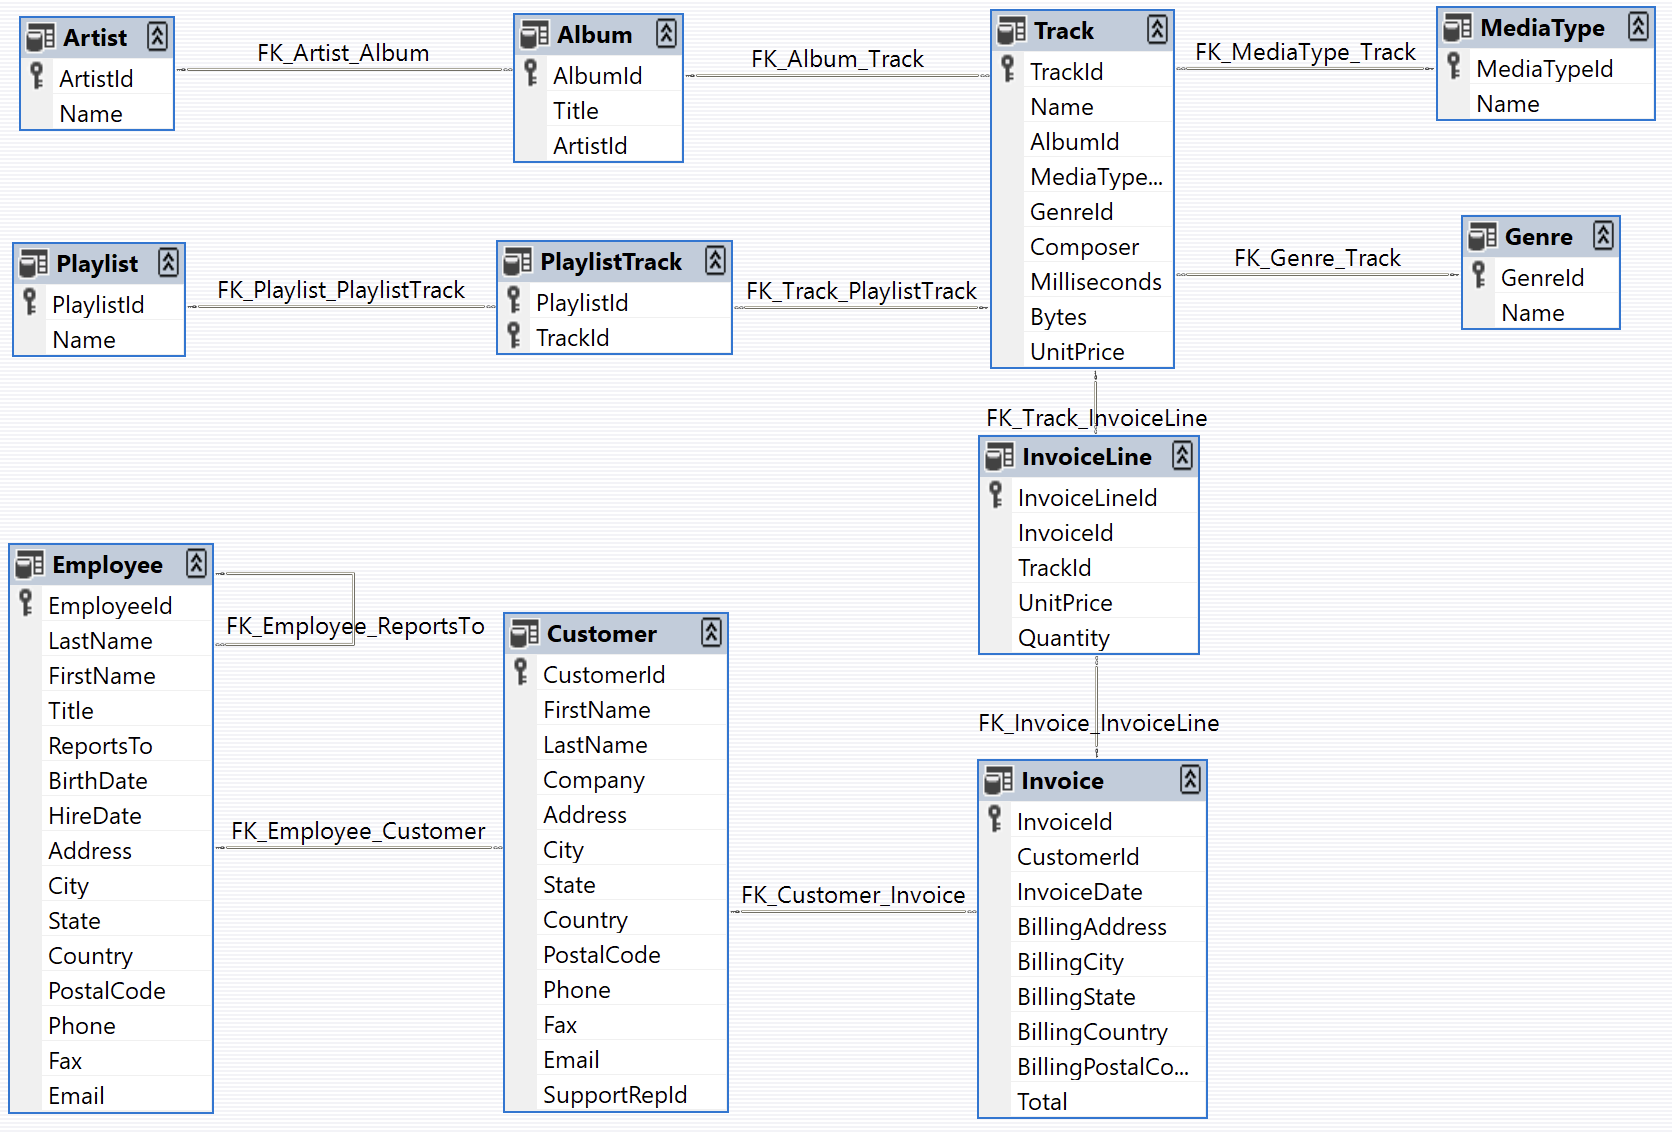
\includegraphics[width=0.8\textwidth]{images/ER_Chinook.png}
    \caption{Schema del database Chinook}
    \label{fig:chinook_schema}
\end{figure}

\begin{figure}[H]
    \centering
    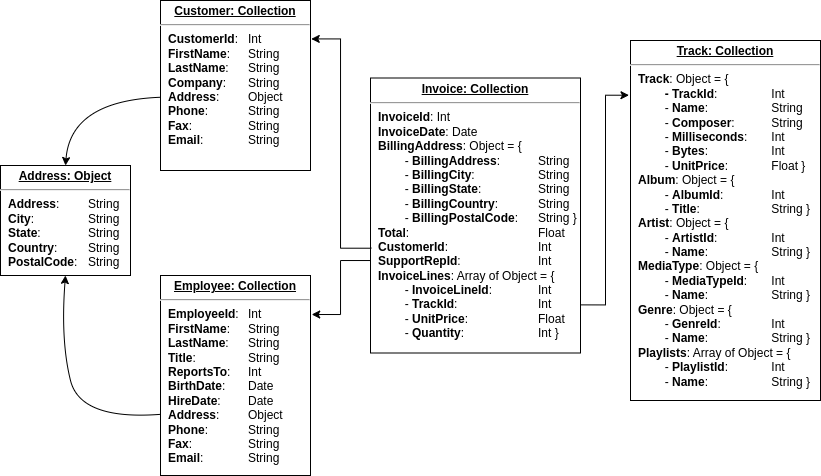
\includegraphics[width=0.8\textwidth]{images/ChinookNoSQL.drawio.png}
    \caption{Schema del database Chinook NoSQL}
    \label{fig:chinook_nosql_schema}
\end{figure}

\subsection{Trasformazione del database}

Come introdotto nella sottosezione precedente, il database originale è stato trasformato in un formato adatto
a un database NoSQL, puntando a ridurre il numero di join e a sfruttare la potenza e la flessibilità di MongoDB.
Per ridurre il numero di join durante le query, le informazioni relative alla musica sono state incorportate in un unico documento per ogni traccia
presente nel database. Questo approccio genera rindondanza, nel senso che ogni albub, ogni artista e ogni genere viene salvato
più volte, una pper ogni traccia, ma permette di ridurre il numero di operazioni con l'operatoe \texttt{\$lookup} e di velocizzare le operazioni di lettura, essendo questo il più costoso.

Per quanto riguarda le informazioni relative a clienti, impiegati e fatture, sono state create tre collezioni separate. La motivazione è che ogni fattura si collega a un cliente, un impiegato e un certo numero di tracce musiciali
in base all'acquisto. Creare una collezione unica per le fatture avrebbe implicato la rindondanza delle informazioni relative a clienti e impiegati, contenenti una discreta quantità di dati. Questo approccio permette quindi 
di risparmiare spazio e effettuare un piccolo numero di join, non ottimale ma le prestazioni non ne risentono nella maggior parte dei casi.

Per inserire i dati nel database sono stati utilizzati due script python, uno che fornisce delle funzioni per la connessione a MongoDB in vari casi: locale, remoto o in Docker, e uno che si occupa di trasformare i dati 
da formato CSV a formato JSON, per poi inserirli nel database. Il codice sorgente per la connessione a MongoDB si trova nel file \textit{db\_utils.py} mentre il codice per la trasformazione del database si trova nel file
\textit{transform\_db.py}. 

\subsection{Interrogazione del database}

Per rendere il progetto fruibile e per permettere di interrogare il database in modo semplice e veloce è stata sviluppata un'interfaccia grafica tramite la libreria Streamlit, una libreria Python che permette di creare
applicazioni web in modo semplice e veloce. L'applicazione si compone di tre pagine, rappresentate da tre file Python:
\begin{itemize}
    \item \textit{app.py}: pagina principale, reindirizza alle altre due pagine in base alla scelta dell'utente
    \item \textit{music.py}: pagina dedicata alla musica, permette di interrogare il database per ottenere informazioni su tracce, album e artisti
    \item \textit{sales.py}: pagina dedicata alle vendite, permette di interrogare il database per ottenere informazioni su fatture, clienti, impiegati e statistiche di vendite
\end{itemize}

Per avviare l'applicazione fare riferimento al file \textit{README.md} presente nel repository. 

\subsubsection{nterrogazione della musica}
La pagina dedicata alla musica permette di interrogare il database per ottenere informazioni su tracce, album e artisti. In particolare offre la possibilità di effettuare
tre tipi di query: contare, raggruppare e contare, filtrare. 

Per quanto riguarda le query di conteggio, è possibile contare il numero di tracce, album, artisti, playlist e generi.

Per le query di raggruppamento invece è possibile contare: 
\begin{itemize}
    \item numero di tracce per album
    \item numero di tracce per genere
    \item numero di tracce per artista
    \item numero di tracce per playlist
    \item numero di artisti per playlist
    \item numero di album per artista
\end{itemize}

La parte dedicata al filtaggio invece è più complessa e permette di creare filtri personalizzati per ricercare tracce, albubm, artisti e qualsiasi dato presente nel database. L'esempio mostrato in Figura~\ref{fig:filtering}
mostra ad esempio una serie di filtri che vanno a cercare tutte le tracce che hanno come artista "AC/DC" e che hanno una lunghezza compresa tra i 3 minuti e i 4 minuti. Inoltre è possibile selezionare
le informazioni da visualizzare, come ad esempio il costo della traccia, il genere, il nome dell'album, ecc. Questo strumento permette di creare query di ricerca personalizzate, concatendando i vari filtri.

\begin{figure}[H]
    \centering
    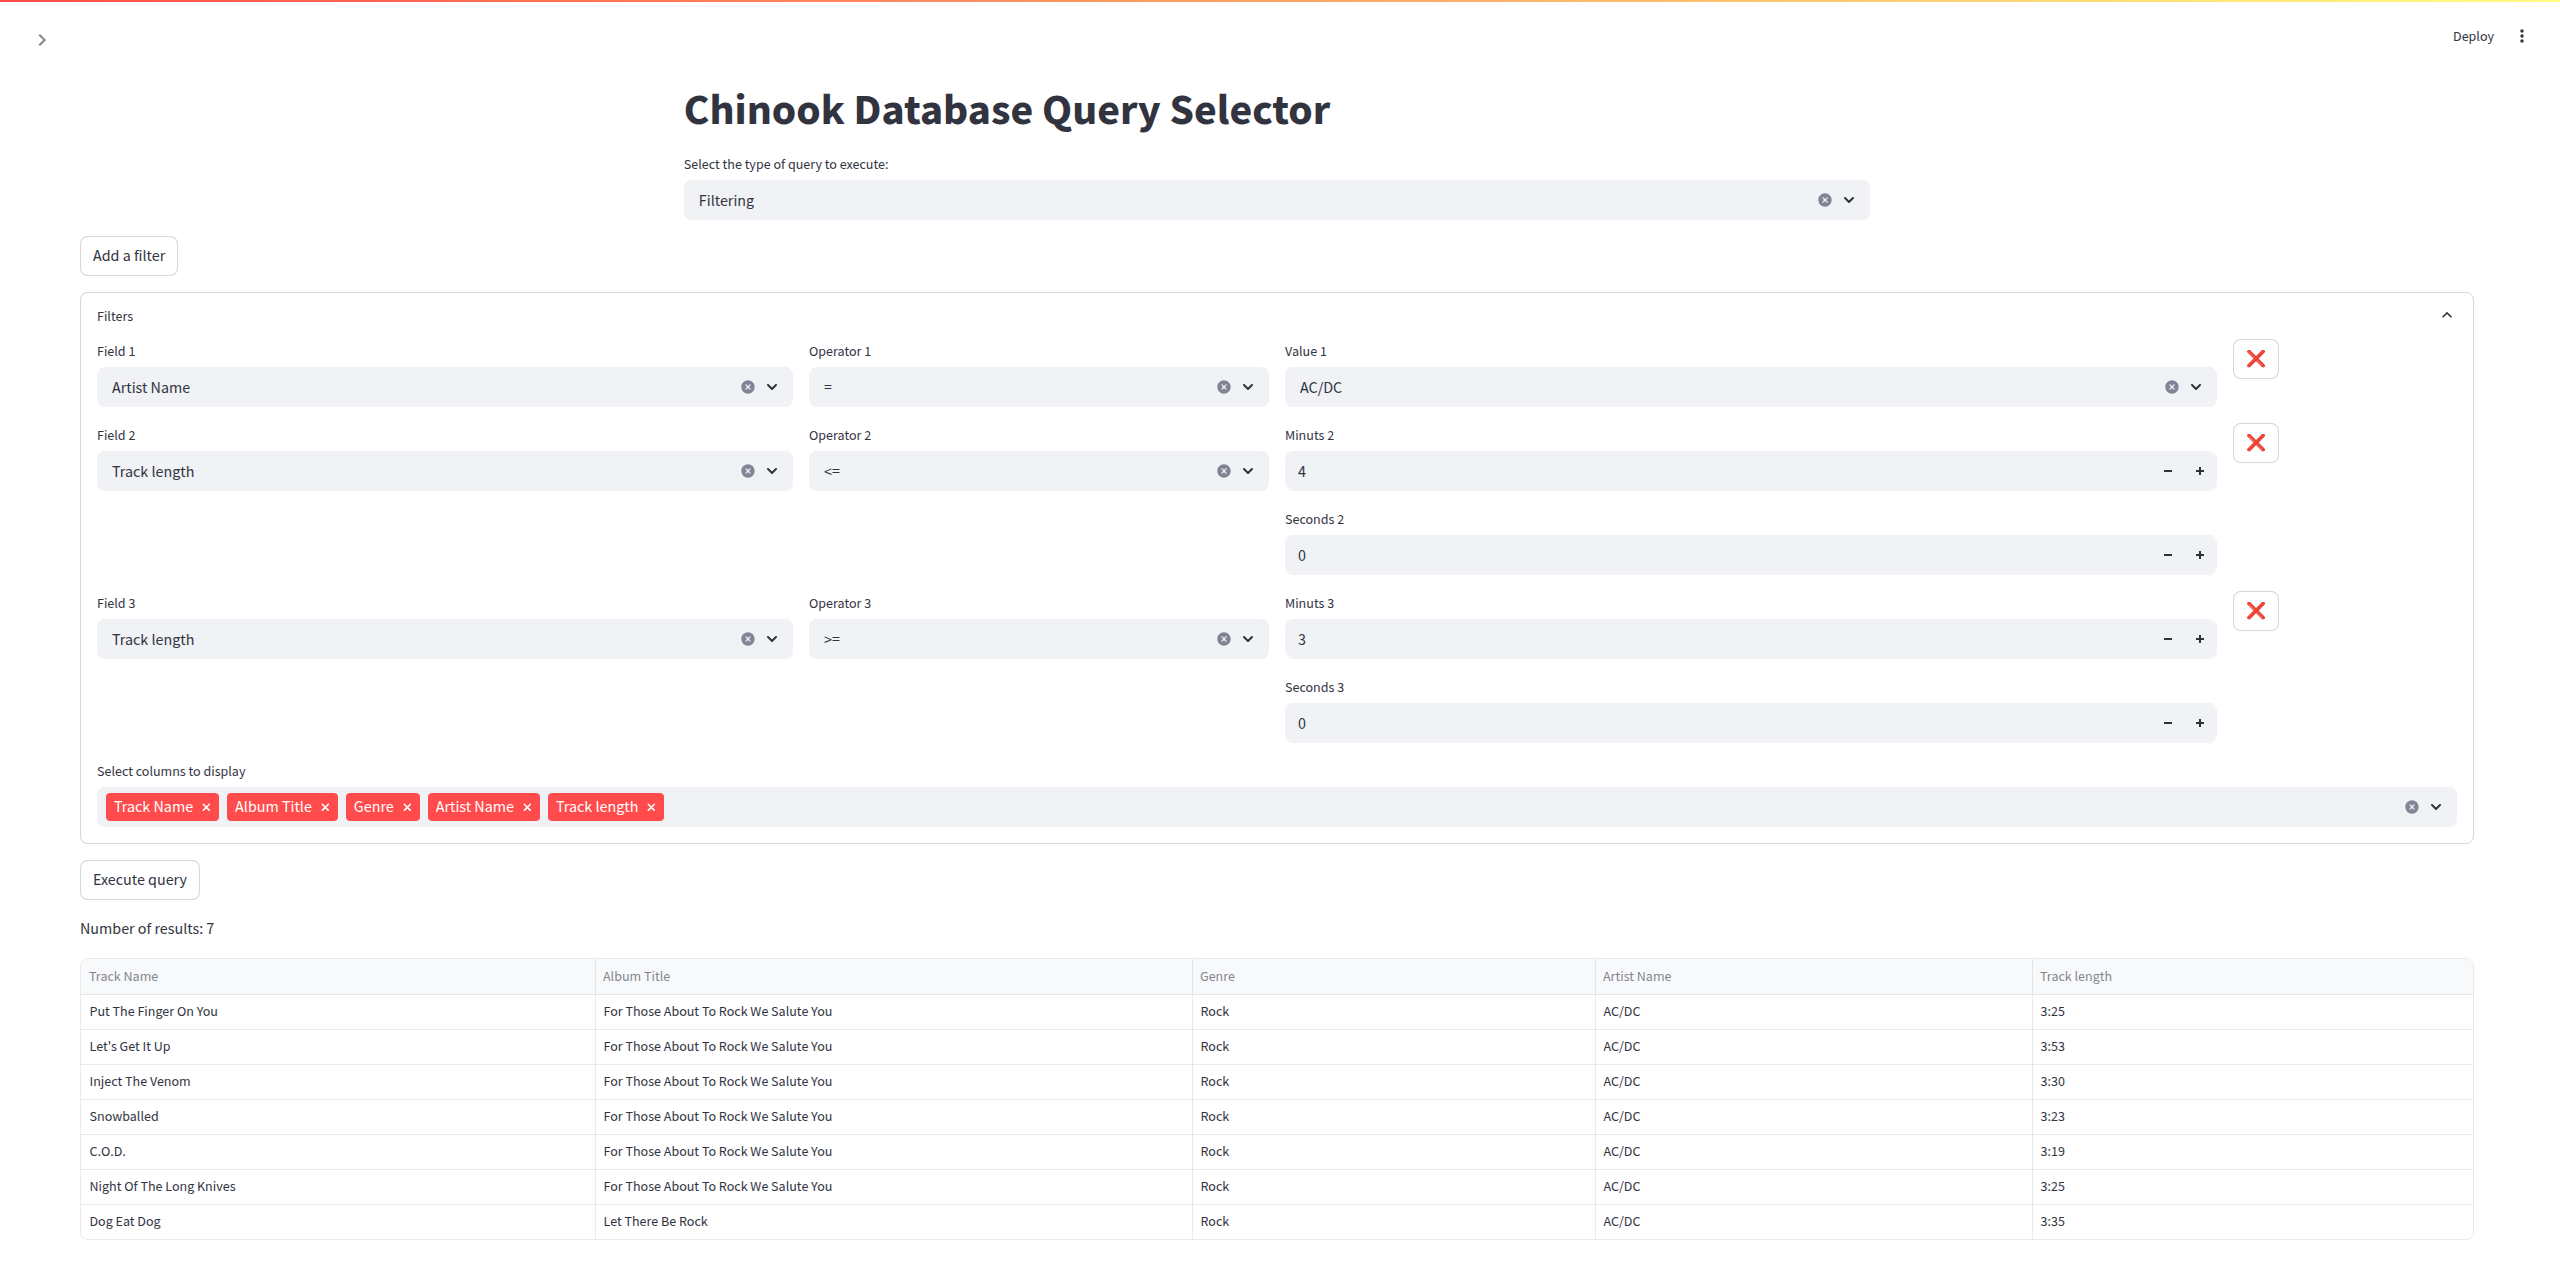
\includegraphics[width=0.8\textwidth]{images/screen_filtering.png}
    \caption{Esempio di filtri per la musica}
    \label{fig:filtering}
\end{figure}



\newpage
\addcontentsline{toc}{section}{References}
\bibliographystyle{apalike}
\bibliography{ref}

\newpage
\appendix
\section{Trasformazione del database}
\label{sec:Trasformazione}
Il codice nel Listato \ref{lst:connessione_mongo} mostra le funzioni per la connessione a MongoDB, in ambiente Docker, in locale o su MongoDB Atlas.
\begin{lstlisting}[language=Python, caption={Connessione a MongoDB}, label={lst:connessione_mongo}]
from pymongo.mongo_client import MongoClient
from pymongo.server_api import ServerApi

def get_docker_connection():
    url = "mongodb://mongodb:27017/"
    client = MongoClient(url)
    # controlla se esiste il db Chinook
    db = client['Chinook']
    # elimina il db Chinook se esiste
    if db in client.list_database_names():
        client.drop_database(db)
    return db["Chinook"]

def get_remote_connection():
    uri = st.secrets['mongo']['uri']
    client = MongoClient(uri, server_api=ServerApi('1'))
    return client['Chinook']

def get_local_connection():
    url = "mongodb://localhost:27017/"
    client = MongoClient(url)
    return client['Chinook']

def pin_g_mongo(client):
    try:
        client.admin.command('ping')
    except Exception as e:
        return False
    return True
\end{lstlisting}

\begin{lstlisting}[language=Python, caption={Inserimento della collezione Track}, label={lst:trasformazione}]

if os.environ.get('DOCKER_BUILD') == 'True':
    db = get_docker_connection()
else:
    db = get_local_connection()

Track = db['Track']
Invoice = db['Invoice']
Customer = db['Customer']
Employee = db['Employee']
    
dfs = {}
table_names = ['Album', 'Artist', 'Customer', 'Employee', 'Genre', 
                'Invoice', 'InvoiceLine', 'MediaType',
                 'Playlist', 'PlaylistTrack', 'Track']
path = 'data/ChinookDataset/'
for table in table_names:
    dfs[table] = pd.read_csv(path + table + '.csv')
    dfs[table].index = np.arange(1, len(dfs[table]) + 1)

for i in range(len(dfs['Track'])):
    record = dfs['Track'].loc[i+1]
    entry = {
        "Track": {
            "TrackId": int(record['TrackId']),
            "Name": record['Name'],
        "Composer": record['Composer'],
            "Milliseconds": int(record['Milliseconds']),
            "Bytes": int(record['Bytes']),
            "UnitPrice": float(record['UnitPrice'])
        },
        "Album": {
            "AlbumId": int(record['AlbumId']),
            "Title": dfs['Album'].loc[record['AlbumId']]['Title']
        },
        "Artist": {
            "ArtistId": int(dfs['Album'].loc[record['AlbumId']]['ArtistId']),
            "Name": dfs['Artist'].loc[dfs['Album'].loc[record['AlbumId']]['ArtistId']]['Name']
        },
        "MediaType": {
            "MediaTypeId": int(record['MediaTypeId']),
            "Name": dfs['MediaType'].loc[record['MediaTypeId']]['Name']
        },
        "Genre": {
            "GenreId": int(record['GenreId']),
            "Name": dfs['Genre'].loc[record['GenreId']]['Name']
        },
        "Playlist": [
            {
                "PlaylistId": int(actual_record['PlaylistId']),
                "Name": dfs['Playlist'].loc[actual_record['PlaylistId']]['Name']
            }
            for actual_record in dfs['PlaylistTrack'].loc[dfs['PlaylistTrack']['TrackId'] == (record['TrackId'] + 1)].to_dict(orient='records')
        ]
    }

    Track.insert_one(entry)
\end{lstlisting}

        
\end{document}






%All other official TU Delft colours
\definecolor{donkerblauw}{RGB}{12, 35, 64}
\definecolor{turkoois}{RGB}{0, 184, 200}
\definecolor{blauw}{RGB}{0, 118, 194}
\definecolor{paars}{RGB}{111, 29, 119}
\definecolor{roze}{RGB}{239, 96, 163}
\definecolor{framboos}{RGB}{165, 0, 52}
\definecolor{rood}{RGB}{224, 60, 49}
\definecolor{oranje}{RGB}{237, 104, 66}
\definecolor{geel}{RGB}{255, 184, 28}
\definecolor{lichtgroen}{RGB}{108, 194, 74}
\definecolor{donkergroen}{RGB}{0, 155, 119}
%You can use these to change the hyperlink colour or the colour of the header or whatever. Glück Auf!